\documentclass{article}

\usepackage{times}
\usepackage{geometry}
\geometry{a4paper,left=0.6cm,right=0.7cm,top=1cm,bottom=1cm,columnsep=0.8cm}

\usepackage{fontawesome}
\usepackage[hidelinks]{hyperref}
\usepackage{multicol,paracol,tikz,hyphsubst,moresize,hyphenat,adjustbox,tabularx,xcolor,enumitem}
\newcolumntype{Y}{>{\RaggedRight\arraybackslash}X}
\setlist[itemize]{itemsep=1pt,leftmargin=*,topsep=-10pt}

\definecolor{maincolor}{HTML}{ffffff}
\definecolor{seccolor}{HTML}{0b1f3b}
\definecolor{gray}{HTML}{8c94a9}
\definecolor{sidetext}{HTML}{59cee5}
\definecolor{Green}{HTML}{2caf00}
\definecolor{lightgray}{HTML}{D3D3D3}

% --- bande latérale bleue
\usepackage{eso-pic}
\AddToShipoutPictureBG{%
  \begin{tikzpicture}[remember picture,overlay]
    \fill[seccolor] (0.7\paperwidth,0) rectangle (\paperwidth,\paperheight);
    \fill[maincolor] (0,0) rectangle (0.7\paperwidth,\paperheight);
  \end{tikzpicture}%
}

\setlength{\parindent}{0pt}
\newcommand{\cvsection}[1]{%
  \par\bigskip                % espace avant le titre
  {\bfseries\Large #1}\par
  \noindent\rule{\linewidth}{0.8pt}\par
  \medskip                    % espace après la ligne
}

\newcommand*{\ClipSep}{0.4cm}

% ------------------------------------------------------------------
\begin{document}\pagestyle{empty}
\columnratio{0.7}\begin{paracol}{2}

% --------- colonne gauche -----------------------------------------
\begin{minipage}{0.7\linewidth}
{\LARGE\textbf{Pape Saliou Fall}}

\bigskip
{\large\textbf{Ingénieur Data Scientist \& Développeur IA}}
\end{minipage}\hfill
\begin{minipage}{0.18\linewidth}
\begin{tikzpicture}
\node[inner sep=0pt]{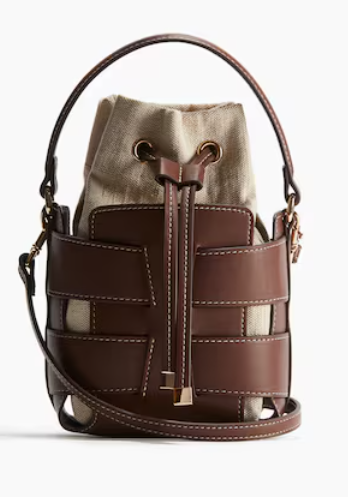
\includegraphics[width=\linewidth]{60db75b75b2547268adad476c1172c78.png}};
\draw[white,rounded corners=\ClipSep,line width=\ClipSep]
      (current bounding box.north west) --
      (current bounding box.north east) --
      (current bounding box.south east) --
      (current bounding box.south west) -- cycle;
\end{tikzpicture}
\end{minipage}

\cvsection{Profil}
Ingénieur Data Scientist et développeur IA, je transforme des ensembles de données complexes en applications intelligentes et rentables. Autonome et proactif, j’aime collaborer avec des équipes pluridisciplinaires pour concevoir des solutions innovantes et industrialisables. Mon expertise couvre le machine learning, le deep learning et l’analyse de séries temporelles, soutenue par une solide culture logicielle et DevOps. Je recherche aujourd’hui un environnement dynamique qui valorise l’innovation et l’excellence technique.

\cvsection{EXPÉRIENCE}

\colorbox{maincolor}{%
  \begin{minipage}{\linewidth}
    \textbf{Data Scientist \& Développeur IA} \\ Prepaya \\ 01/2024 - Présent
    \begin{itemize}
      \item Conçu une plateforme IA en Python/JavaScript intégrée à l’API OpenAI et déployée sur Heroku. \item Implémenté des modèles de machine et deep learning pour l’analyse de séries temporelles, améliorant la précision prédictive. \item Structuré la base PostgreSQL et les pipelines Flask/Scikit-learn pour un déploiement continu.
    \end{itemize}
  \end{minipage}}

\vspace{3mm}


\colorbox{maincolor}{%
  \begin{minipage}{\linewidth}
    \textbf{Apprenti Risk Analyst \& Data Scientist} \\ AXA XL (Groupe AXA) \\ 12/2022 - 12/2023
    \begin{itemize}
      \item Automatisé la collecte et l’intégration des données financières, réduisant le temps de traitement. \item Créé des tableaux de bord Power BI facilitant le suivi de la facturation pour finance et management. \item Développé des modèles de prédiction de sinistres en Python/VBA, renforçant la gestion du risque.
    \end{itemize}
  \end{minipage}}

\vspace{3mm}


\colorbox{maincolor}{%
  \begin{minipage}{\linewidth}
    \textbf{Apprenti Data Scientist} \\ Prepaya \\ 09/2021 - 08/2022
    \begin{itemize}
      \item Mis en œuvre des modèles NLP avancés (T5, BERT) pour générer automatiquement des formulaires clients. \item Réalisé des analyses de sentiment sur les retours utilisateurs afin de guider les actions marketing. \item Automatisé la collecte web avec Python/BeautifulSoup et Selenium pour alimenter les jeux de données.
    \end{itemize}
  \end{minipage}}

\cvsection{FORMATION}

    \begin{tabularx}{\linewidth}{@{}c X@{}}
    \textcolor{sidetext}{\faGraduationCap} &
    \textbf{Master 2 Data Science} \\
    & Sorbonne Université, Paris \\
    & \begin{itemize}[leftmargin=*]
  \item Approfondissement en analyse de données, machine learning et deep learning. \item Études de séries temporelles, modèles de structure latente et apprentissage statistique. \item Projets pratiques sur bases de données, calcul parallèle et déploiement de modèles.
\end{itemize} \\
    & \textit{09/2021 - 03/2022}
    \end{tabularx}
    

% --------- colonne droite (bleue) ---------------------------------
\switchcolumn\color{white}\hspace*{0.4cm}\begin{minipage}{0.88\linewidth}

\cvsection{CONTACT}
\begin{tabular}{@{}c l}
  \faPhone & \href{tel:0753481453}{0753481453} \\[2pt]
  \faEnvelope & \href{mailto:papesalioufall2@gmail.com}{papesalioufall2@gmail.com} \\[2pt]
  \faMapMarker & 95300 Pontoise\\ \\[2pt]
  \faLinkedin & \href{https://www.linkedin.com/in/pape-saliou-fall-43154a211}{pape-saliou-fall-43154a211}
\end{tabular}

\cvsection{COMPÉTENCES}

\begin{itemize}[leftmargin=*]
\item Python
\item JavaScript
\item SQL
\item Tensorflow
\item Scikit
\item PowerBI
\item Git\end{itemize}
\par\bigskip 

\cvsection{LANGUES}
\begin{itemize}[leftmargin=*]
\item Français - \textcolor{gray}{Natif}
\item Anglais - \textcolor{gray}{B2}\end{itemize}
\par\bigskip 
\cvsection{CENTRES D’INTÉRÊT}
\begin{itemize}[leftmargin=*]
\item Football
\item Natation
\item Lecture
\end{itemize}

\end{minipage}
\end{paracol}
\end{document}
